\documentclass[12pt]{article}
\usepackage[shortlabels]{enumitem}
\usepackage{graphicx}
\begin{document}
\title{TCSS 343 - Week 4}
\author{Jake McKenzie}
\maketitle
\noindent\centerline{\textbf{Homework 2}}
\\\\3.5 When a process creates a new process using the fork() operation, which
of the following states is shared between the parent process and the child
process?\\\\
\textbf{ANSWER: } \\c. Shared memory segments. Processes can only share read-only memory or
create shared-memory regions of safe memory(I was confused by the latter but you 
mentioned this in class. The book was unclear on this point). 
It would make no sense for the processes to 
share a stack or heap. \\\\
3.9 Describe the actions taken by a kernel to context-switch between
processes.\\\\
\textbf{ANSWER: } \\
Say we have two processes $P_1$ and $P_2$. Their process control blocks 
reside in memory and the values of the CPU will change depending on which process is 
currently executing. A context is the mechanism used for switching the CPU from 
the context of one process to the context of another. When the operating system 
switches from the execution of $P_1$ $\rightarrow$ $P_2$ and again
when the operating system switches from the execution of 
$P_2$ $\rightarrow$ $P_1$. This operation can be expensive. There are both 
direct and indirect costs. The direct cost includes cycling for loading and
storing of instructions. The indirect costs from cold cache(cache misses).\\

\noindent In modern CPUs there exists a cache hierarchy. Accessing this cache is many 
orders of magnitude faster than accessing memory. Using our $P_1$, $P_2$ process
from before. Say the data for $P_1$ is in the cache, we would say in this case 
that the cache is hot but say we context switch $P_1$ $\rightarrow$ $P_2$ and we 
need to access the data for $P_2$ which is not in the cache. In this case we would say 
the cache is cold. Not only do we need to retrieve the data for $P_2$ and put it into 
the cache but we need to replace the data for $P_1$ in the cache with that of $P_2$.\\

\noindent Long story short, having a cold cache sucks. The hotter your cache, the smoother 
your OS operates so limiting the number of context switching is optimal.\\\\
3.10 Construct a process tree similar to Figure 3.8. To obtain process information
for the UNIX or Linux system, use the command ps -ael.\\
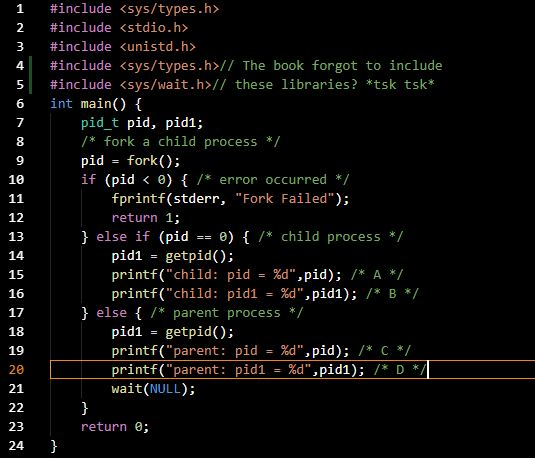
\includegraphics[scale = .7]{code.jpg}\\
Use the command man ps to get more information about the ps command.
The task manager on Windows systems does not provide the
parent process ID, but the process monitor tool, available from technet.
microsoft.com, provides a process-tree tool.\\\\
\textbf{ANSWER: }\\\\
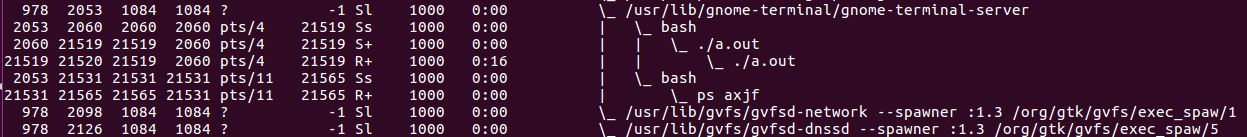
\includegraphics[width=1\textwidth]{tree.jpg}\\
I apologize if it's tiny but we can clearly see that my program generated a child 
from a parent. The parent has a PID of 21519 whie the child has a PPID of that is 
the same. \\\\
3.12 Including the initial parent process, how many processes are created by
the program shown in Figure 3.32?\\\\
\textbf{ANSWER: }\\
So at each interation of the loop we fork() we fork once. This will make 4
parents. This process creates a binary tree which gives us the following 
equation for the problem: $\sum\limits_{i=0}^{3}{2^i} + 1=2^4-1 + 1=16$. \\\\
3.13 Explain the circumstances under which the line of code marked
printf("LINE J") in Figure 3.33 will be reached.\\\\
\textbf{ANSWER: }\\
If the process generated from fork() is a child then this line will have been 
reached. There must have been an error to reach this stage.\\\\
3.14 Using the program in Figure 3.34, identify the values of pid at lines A, B,
C, and D. (Assume that the actual pids of the parent and child are 2600
and 2603, respectively.)\\\\
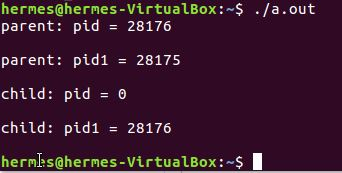
\includegraphics[width=1\textwidth]{q_pi.jpg}\\
3.17 Using the program shown in Figure 3.35, explain what the output will
be at lines X and Y.\\\\
\textbf{ANSWER: }\\\\
Whenever a child is produced it generates $0*(-0)$ then $1*(-1)$ then $2*(-2)$ 
then $3*(-3)$ then $4*(-4)$ producing:\\ 
$X = \{0, -1, -4, -9, -16\}$\\\\
Whenever a parent is produced it generates the following list:\\
$Y = \{0, 1, 2, 3, 4\}$\\
\textbf{Extra Credit}\\\\
The following exercise is optional and it has two project points: We 
discussed this function in class. It forks and runs a program. Make 
an independent program of this code and name it “execute”. Use “execute” 
to run your “copy” program. Make the necessary changes in the given 
code.\\\\
\textbf{ANSWER: }\\\\
I will include the file I used to produce this output as well. I didn't 
like the code included from the book. I felt it was clunky and over complicated 
so I wrote my own. Thank you and I hope you have a good day whenever you get to 
this. :)\\\\
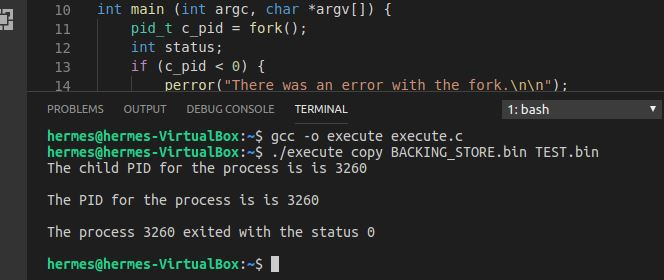
\includegraphics[width=1\textwidth]{extracredit.jpg}\\
\end{document}